\documentclass[a4paper]{article}

\usepackage[portuguese]{babel}
\usepackage[utf8]{inputenc}
\usepackage{amsmath}
\usepackage{graphicx}
\usepackage{subfigure}
\usepackage{float}
\usepackage{listings}
\usepackage{multirow}
\usepackage{booktabs}
\usepackage[table,xcdraw]{xcolor}
\usepackage[numbered, framed]{mcode}
\usepackage[colorinlistoftodos]{todonotes}

\title{ \textbf {Implementação do classificador Bayesiano utilizando MATLAB} }

\author{Gustavo Siebra Lopes\thanks{gustavosiebra@gmail.com}} 


\date{\today}


\begin{document}


\maketitle


\section{Introdução}

Esse trabalho é para compor a nota na disciplina de Aprendizagem de Máquina. Consiste na implementação do código para diferentes bases usando MATLAB, um breve relatório sobre as técnicas de reconhecimento de padrão utilizada e seus resultados.


\section{Preparação da base}

As bases utilizada nesse relatório estão disponibilizadas na UCI Machine Learning Repository.[1]

\subsection{Base de dados da Flor de Íris}

Nessa base são definidas 3 classes (Iris Setosa, Iris Versicolour, Iris Virginica) e 4 parametros por classe (comprimento e largura da sépala e pétala). A base possui 150 padrões diferentes de Iris dividido em 50 para cada classe.

\subsubsection{Análise das características}
\label{sec:examples}

Na figura \ref{fig:Figura1} é apresentada a matriz de características. Essa matriz consiste de gráficos formados pelos pares de características combinadas.


\begin{figure}[H]
\centering

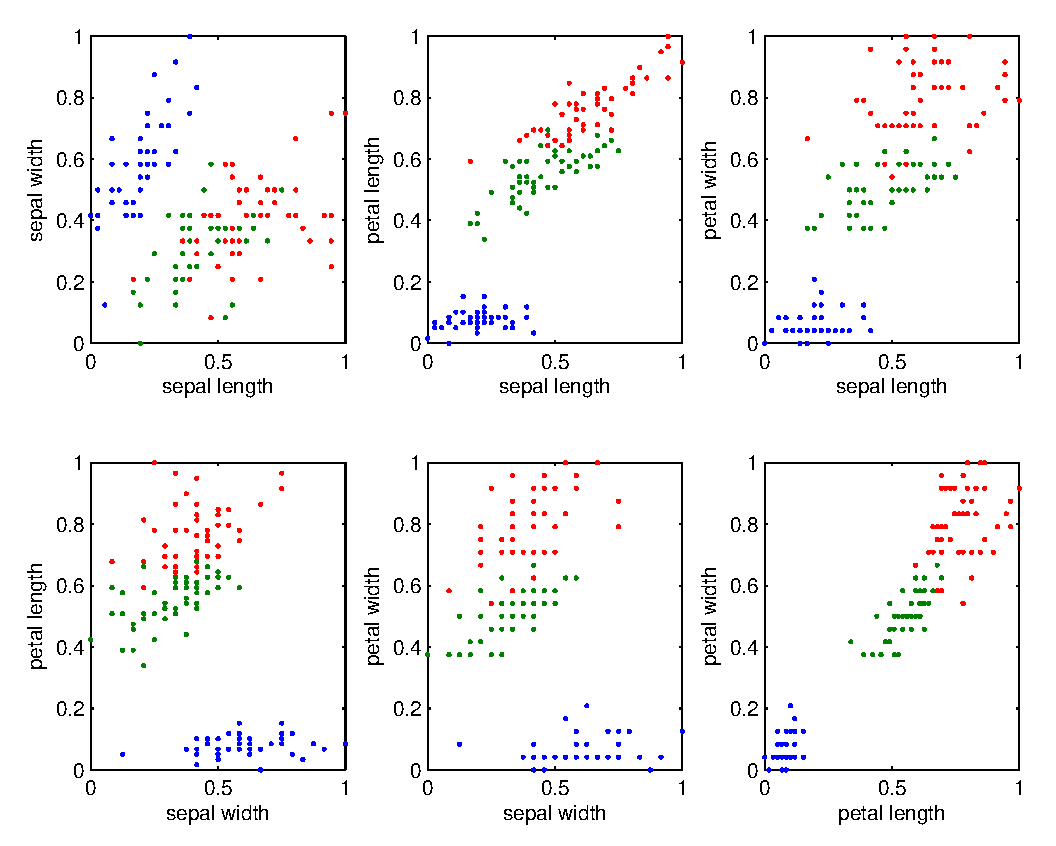
\includegraphics[height=9cm]{Imagens/myfig.eps}


\caption{Matriz de características.}
\label{fig:Figura1}
\end{figure}

Podemos perceber que a classe setosa pode facilmente ser separada das outras utilizando a largura ou o comprimento da pétala como variável, já para as duas outras características essa separação não é tão simples, perceba a sobreposição dos histogramas em todos os atributos bem como a mistura das classes nos gráficos de dispersão.


\subsection{Base de dados da Dermatologia}

Esta base de dados contém 34 atributos, 33 dos quais são valorizados linear e um deles é nominal. O diagnóstico diferencial das doenças eritêmato-escamosas é um problema real em dermatologia. Todos eles compartilham as características clínicas de eritema e descamação, com poucas diferenças. As doenças deste grupo são a psoríase, dermatite seboreic, líquen plano, pitiríase rósea, dermatite crônica, e pitiríase rubra pilar. Geralmente é necessário para o diagnóstico de uma biópsia, mas infelizmente essas doenças compartilham muitas características histopatológicas. Uma outra dificuldade para o diagnóstico diferencial é uma doença que pode apresentar as características de uma outra doença na fase inicial e pode ter as características específicas nas fases seguintes. Os pacientes foram avaliados clinicamente primeiro com 12 recursos. Depois disso, amostras de pele foram levados para a avaliação de 22 características histopatológicas. Os valores das características histopatológicas são determinadas por uma análise das amostras sob um microscópio. \\

No conjunto de dados construída para este domínio, o recurso história familiar tem o valor 1, se qualquer uma destas doenças tem sido observado na família, e 0, caso contrário. A característica idade representa simplesmente a idade do paciente. Cada outro recurso (clínico e histopatológico) foi dado um grau na escala de 0 a 3. Aqui, 0 indica que o recurso não estava presente, 3 indica a maior quantidade possível, e 1, 2 indicam os valores intermediários relativos.

\subsection{Base de dados da Coluna Vertebral}

Cada paciente é representado no conjunto de dados por seis atributos biomecânicas decorrentes da forma e orientação da pelve e coluna lombar (nesta ordem): incidência pélvica, a inclinação da pelve, ângulo lordose lombar, inclinação sacral, raio pélvica e grau de espondilolistese. A seguinte convenção é utilizada para os rótulos de classe: DH (Disco de Hérnia), espondilolistese (SL), Normal (NO) e anormal (AB).\\

Os dados foram organizados em duas tarefas de classificação diferentes, mas relacionadas. A primeira tarefa consiste em classificar os pacientes como pertencente a uma das três categorias: Normal (100 doentes), Disco de Hérnia (60 pacientes) ou Espondilolistese (150 pacientes). Para a segunda tarefa, as categorias de disco hérnia e espondilolistese foram fundidas em uma única categoria rotulado como "anormal". Assim, a segunda tarefa consiste em classificar os pacientes como pertencendo a uma de duas categorias: Normal (100 doentes) ou anormal (210 pacientes).


\section{Classificador de Bayes}

Classificadores Bayesianos são classificadores estatísticos que classificam um objeto em uma determinada classe baseando-se na probabilidade deste objeto pertencer a esta classe. Produz resultados rapidamente e ótimo no tocante a minimização da probabilidade de erro de classicação.


\subsection{Teorema de Bayes}

Sejam padrões x = $\{x_1, x_2, \cdots, x_m\}$ $\in$ $\Re^d$ e classes $\{w_1, w_2, \cdots, w_m\}$. Em reconhecimento de padrões ou classificação, o interesse está em associar a um padrão uma determinada classe.\\

A abordagem Bayesiana supõe que as probabilidades de cada classe P($w_i$) e as densidades de probabilidade condicionais p(x $\mid$ $w_i$) de x com respeito a cada uma das classes $w_i$ = $\{1, 2, \cdots, c\}$ são conhecidas.\\

O classificador Bayesiano decide pela classe com maior probabilidade P($w_i$$\mid$x) (probabilidade a posteriori). Esta probabilidade é calculada pela regra de Bayes. 

\begin{align}
\text {P($w_i$ $\mid$ x) = $\dfrac{P(w_i) \times p(x \mid w_i)}{p(x)}$}
\end{align}

\begin{align}
\text {p(x) = $\sum_{j=1}^{c}$P($w_j$)p(x $\mid$ $w_j$)}
\end{align}

na qual P($w_i$) é a priori, o p(x) é a pdf (função densidade de probabilidade misturada das classes) e p(x $\mid$ $w_i$) é a função densidade de probabilidade de cada classe $w_i$ . No entanto, o p(x) é a evidência sendo o mesmo para todas as classes. Portanto, o classificador pode selecionar a classe com maior valor $g_i$(x) = P($w_i$)p(x $\mid$ $w_i$)(função critério).\\

Esse classificador pode ser paramétrico e não-paramétrico, no sentido que os paramétricos buscam estimar as densidades de probabilidade da Equação 1 e o não-paramétrico estima a probabiliade a posteriori a partir das amostras em uma dada região R de $\Re^n$.\\

\begin{align}
\text {p(x) = $\frac{1}{(2\pi)^{\frac{d}{2}} \Sigma^{\frac{1}{2}}} \cdot exp\{-\dfrac{1}{2} (x - \mu)^T \Sigma^{-1} (x - \mu)\}$}
\end{align}

A funcão densidade multivariada Gaussiana contínua é dada na Equação 3 em que \textbf{x} é um vetor coluna com \textit{d} componentes, $\mu$ é o vetor de médias também com \textit{d} componentes e $\Sigma$ é a matriz de covariância de tamanho \textit{d}$\times$\textit{d}. Logo, $|\Sigma|$ e $\Sigma^{-1}$ são o determinante e a inversa da matriz de covariância, respectivamente.\\

Nesse relatório é apresentado 4 Funções Discriminantes dado por:

\begin{enumerate}
\item \textbf{Quadrática}: Matriz de covariância diferentes e probabilidades a priori diferentes.

\item \textbf{Linear}: Matriz de covariância diagonal com atributos da mesma variância e probabilidades priori diferentes.

\item \textbf{Distância Euclidiana}: Matriz de covariância diagonal com atributos da mesma variância e probabilidades a priori iguais.

\item \textbf{Mahalanobis}: Matriz de covariância diferentes e probabilidades a priori iguais.
\end{enumerate}


\subsection{Algoritmo}

A base foi dividida usando o modelo holdout. Este método consiste em dividir o conjunto total de dados em dois subconjuntos mutuamente exclusivos, um para treinamento (estimação dos parâmetros) e outro para teste (validação). O conjunto de dados pode ser separado em quantidades iguais ou não. Uma proporção muito comum é considerar 2/3 dos dados para treinamento e o 1/3 restante para teste. [3]\\

Após o carregamento da base foi realizado a normalização dos dados separadamente para cada atributo. Identificando o mínimo e o máximo que foram normalizados na faixa [0,1].\\

O algoritmo tem como objetivo calcular a probabilidade que uma amostra desconhecida pertença a cada uma das classes possíveis, ou seja, predizer a classe mais provável. Este tipo de predição é chamada de classificação estatística, pois é completamente baseada em probabilidades. \\

Esse algoritmo requer um conjunto de dados prévio que já esteja classificado, ou seja, um conjunto que já estejam separadas em classes (ou clusters). Baseado neste conjunto de dados prévio, que também é chamado de conjunto de treinamento, o algoritmo recebe como entrada uma nova amostra desconhecida, ou seja, que não possui classificação, e retorna como saída a classe mais provável para esta amostra de acordo com cálculos probabilísticos. O algoritmo deve seguir os seguintes passo:\\


\textbf{Passo 01}: Cálculos das probabilidades das classes.\\

Neste passo, cada classe do conjunto de treinamento possui sua probabilidade calculada. O cálculo é feito dividindo-se o número de instâncias de determinada classe pelo número total de instâncias do conjunto de treinamento.\\

\textbf{Passo 02}: Cálculo das probabilidades da amostra desconhecida.\\

Agora, o valor de cada atributo da amostra desconhecida possui sua probabilidade calculada para cada possível classe. Este passo é onde o processamento mais ‘pesado’ do algoritmo ocorre, pois, dependendo do número de atributos, classes e instâncias do conjunto de treinamento, é possível que muitos cálculos sejam necessários para se obter as probabilidades.\\

É importante notar que este cálculo depende inteiramente dos valores dos atributos da amostra desconhecida, ou seja, da amostra que se deseja prever a classes. Supondo que existam k classes no conjunto de testes e m atributos conjunto de testes será necessário calcular k x m probabilidades.\\

\textbf{Passo 03}: Calcular a probabilidades da amostra desconhecida.\\

Neste passo, as probabilidades calculadas para os valores da amostra desconhecida de uma mesma classe são multiplicadas. Em seguida, o valor obtido é multiplicado pela probabilidade da classe calculada no Passo 01.\\

Com as probabilidades de cada classe calculadas, verifica-se qual é a classe que possui maior probabilidade para a amostra desconhecida. Com isso, o algoritmo termina retornando a classe que possui maior probabilidade de conter a amostra desconhecida.


\section{Resultados}

\subsection{Acurácia}


Acurácia é a proporção de acertos, ou seja, o total de verdadeiramente positivos e verdadeiramente negativos, em relação a amostra estudada. O resultado da acurácia foi obtido através de 25 iterações, realizadas para 4 tipos de funções discriminante. \\

\subsubsection{Flor de Íris}

\begin{figure}[H]
\centering

\subfigure[Quadrática]{ 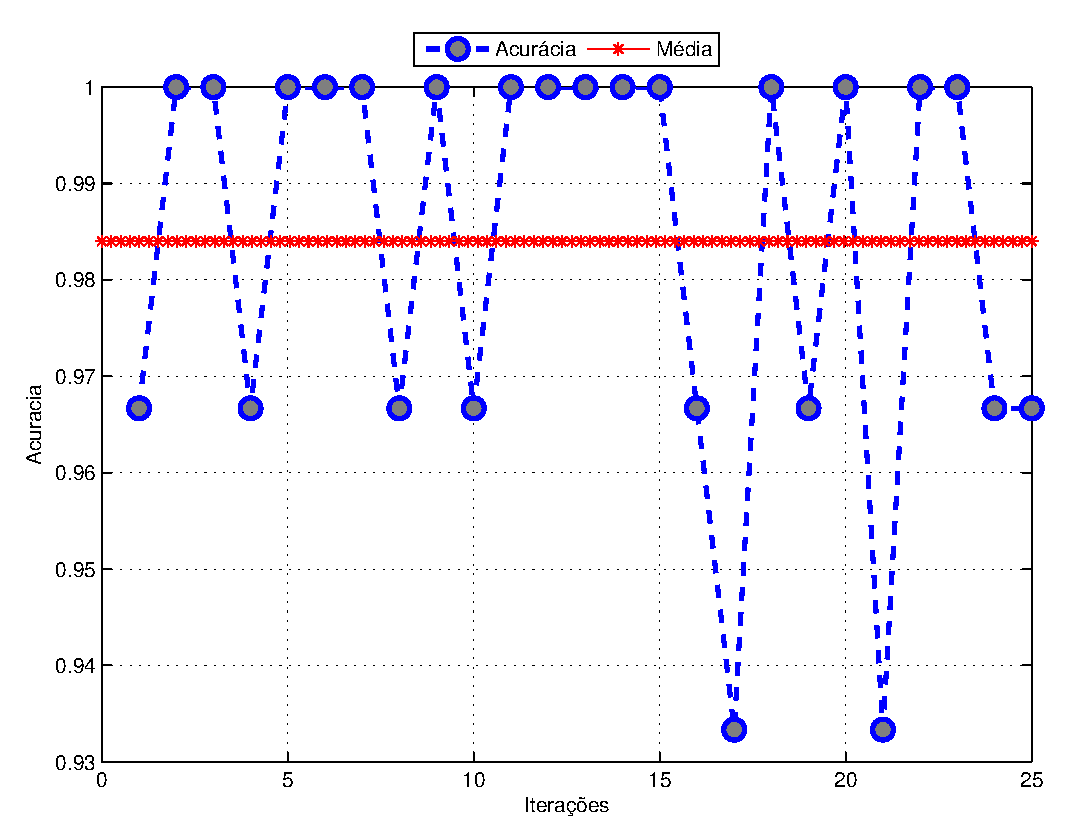
\includegraphics[width=0.4\textwidth]{Imagens/plotAcc_type1.eps}}
\subfigure[Linear]{ 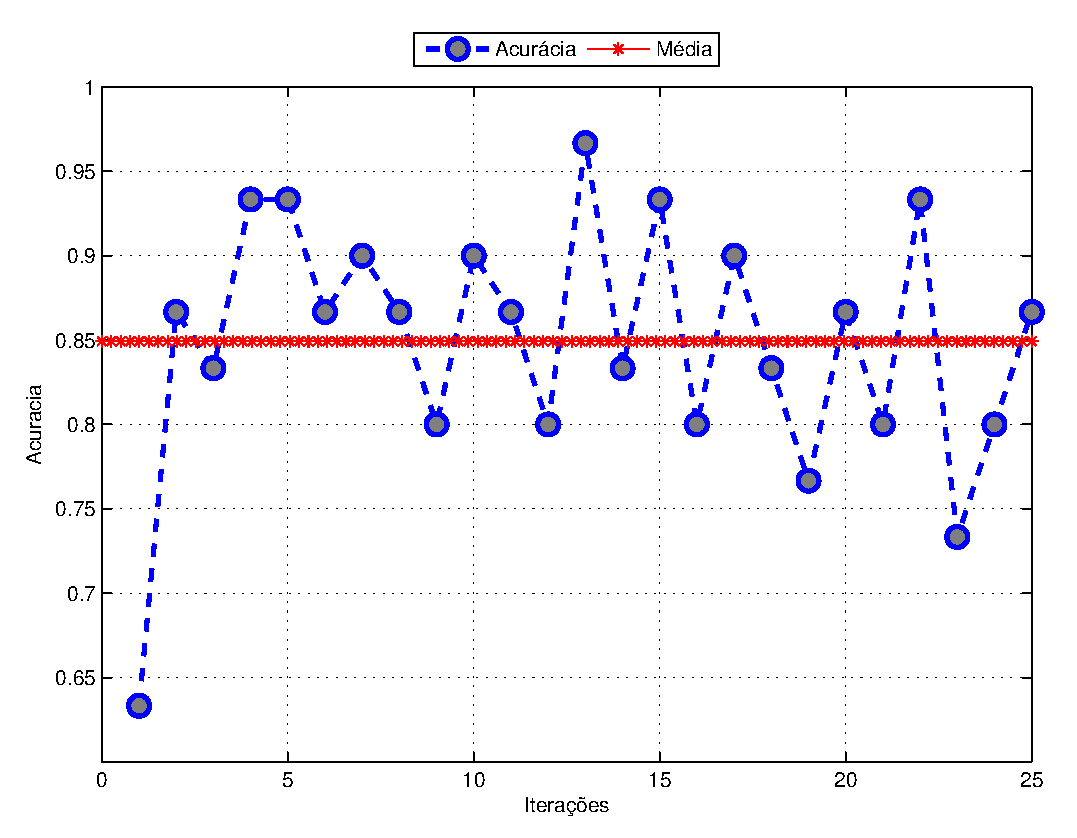
\includegraphics[width=0.4\textwidth]{Imagens/plotAcc_type2.eps}}
\subfigure[Distância Euclidiana]{ 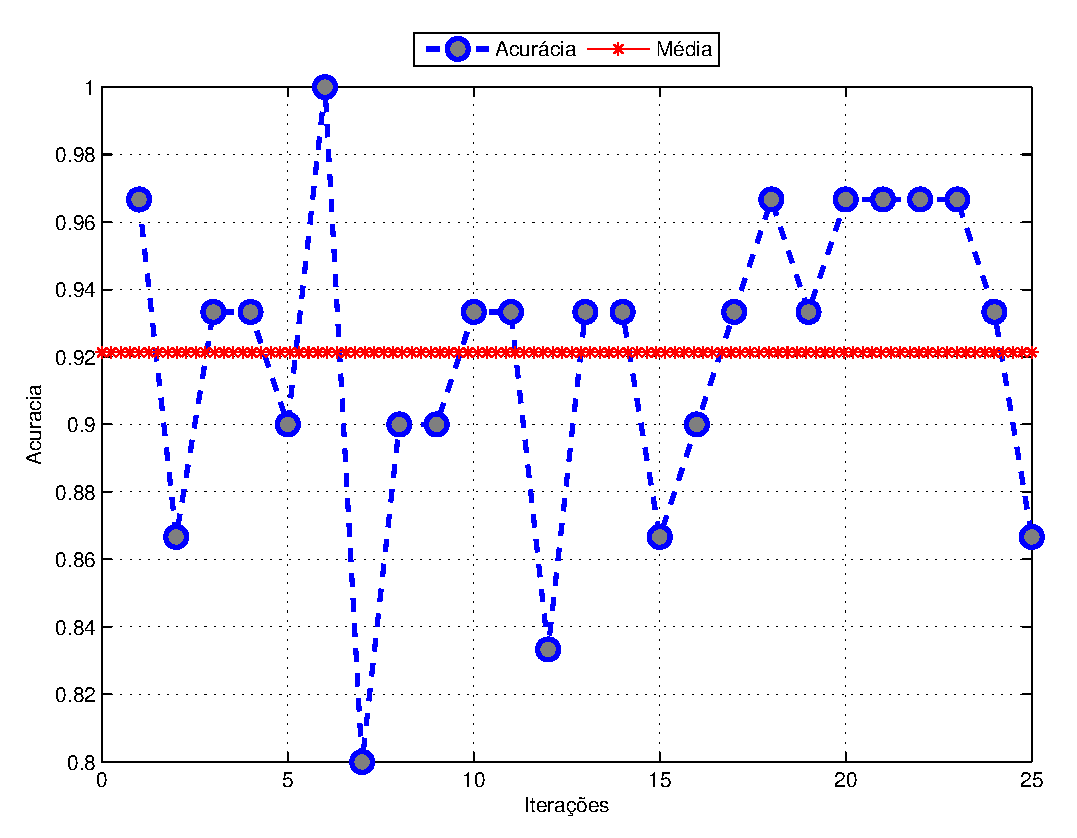
\includegraphics[width=0.4\textwidth]{Imagens/plotAcc_type3.eps}}
\subfigure[Mahalanobis]{ 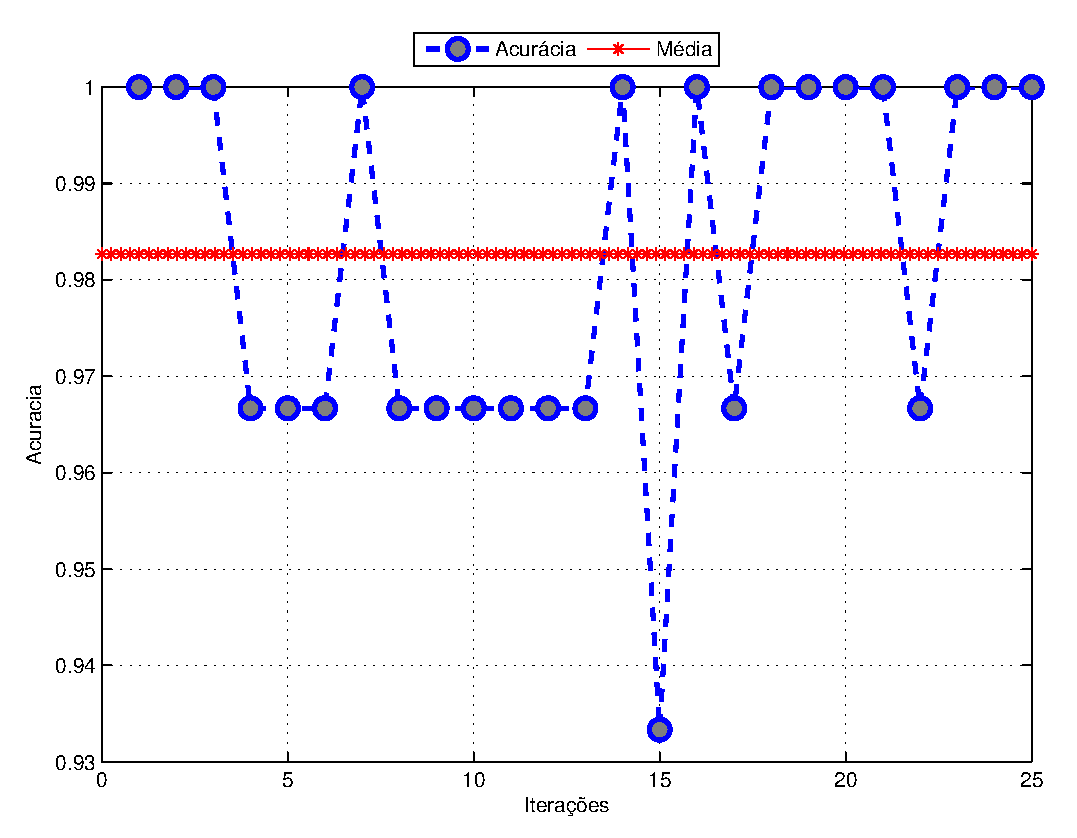
\includegraphics[width=0.4\textwidth]{Imagens/plotAcc_type4.eps}}

\caption{Resultados da Acurácia para Flor de Íris.}
\label{fig:Figura2}
\end{figure}



\subsubsection{Dermatologia}

\begin{figure}[H]
\centering

\subfigure[Quadrática]{ 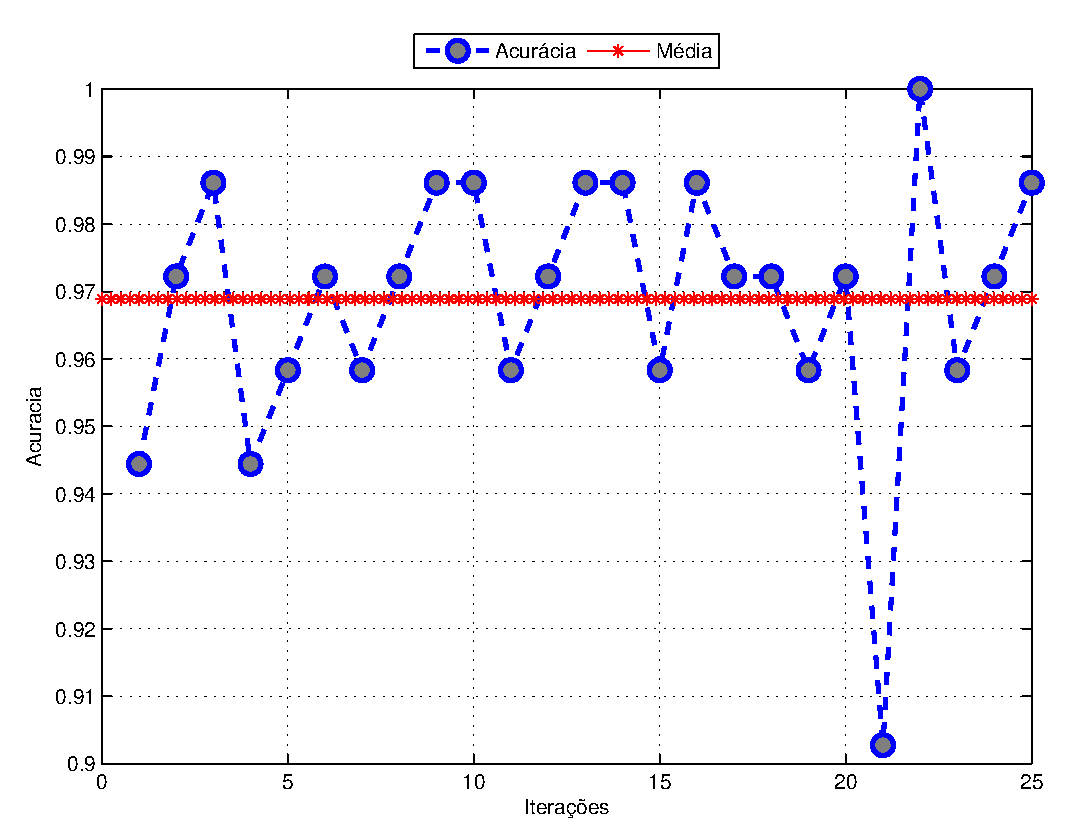
\includegraphics[width=0.4\textwidth]{Imagens/plotAccDerm_type1.eps}}
\subfigure[Linear]{ 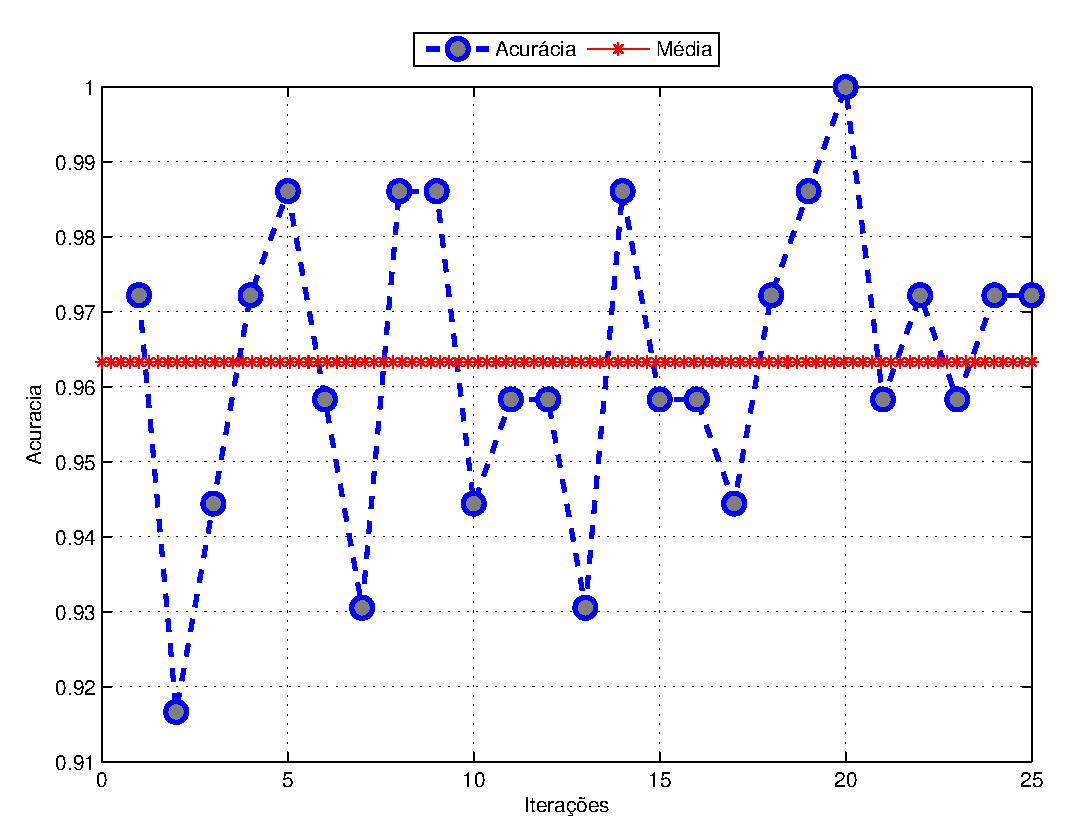
\includegraphics[width=0.4\textwidth]{Imagens/plotAccDerm_type2.eps}}
\subfigure[Distância Euclidiana]{ 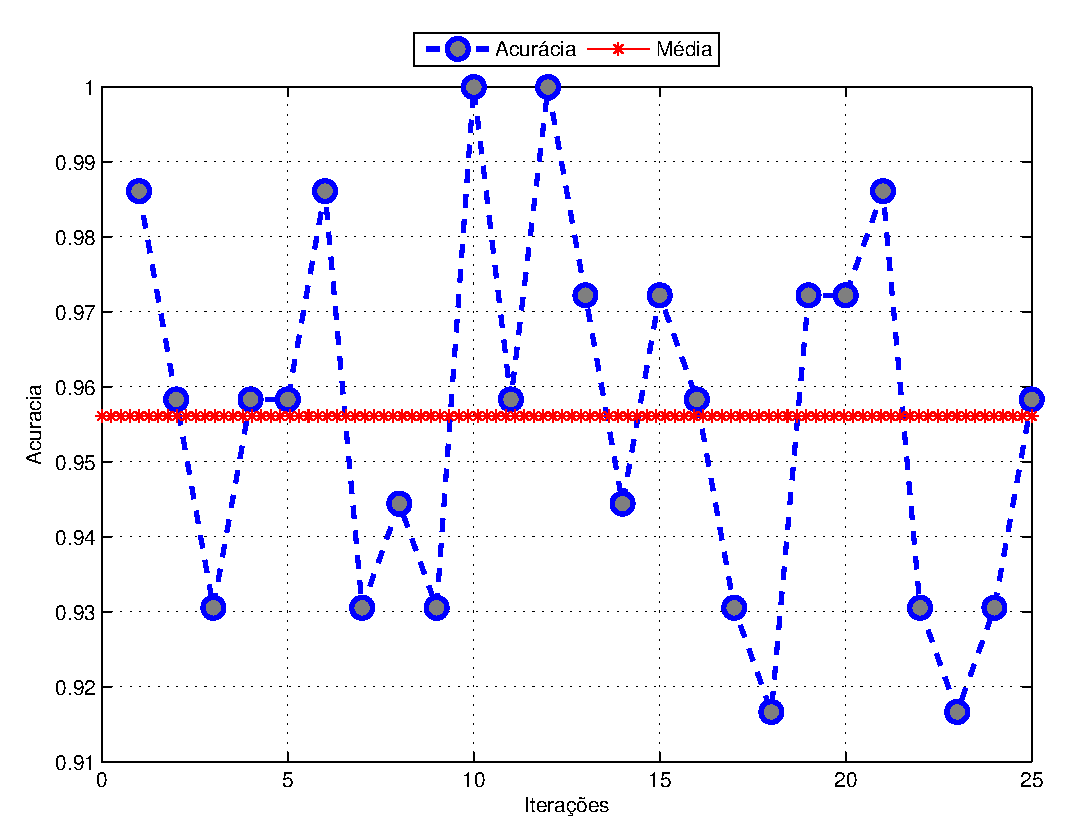
\includegraphics[width=0.4\textwidth]{Imagens/plotAccDerm_type3.eps}}
\subfigure[Mahalanobis]{ 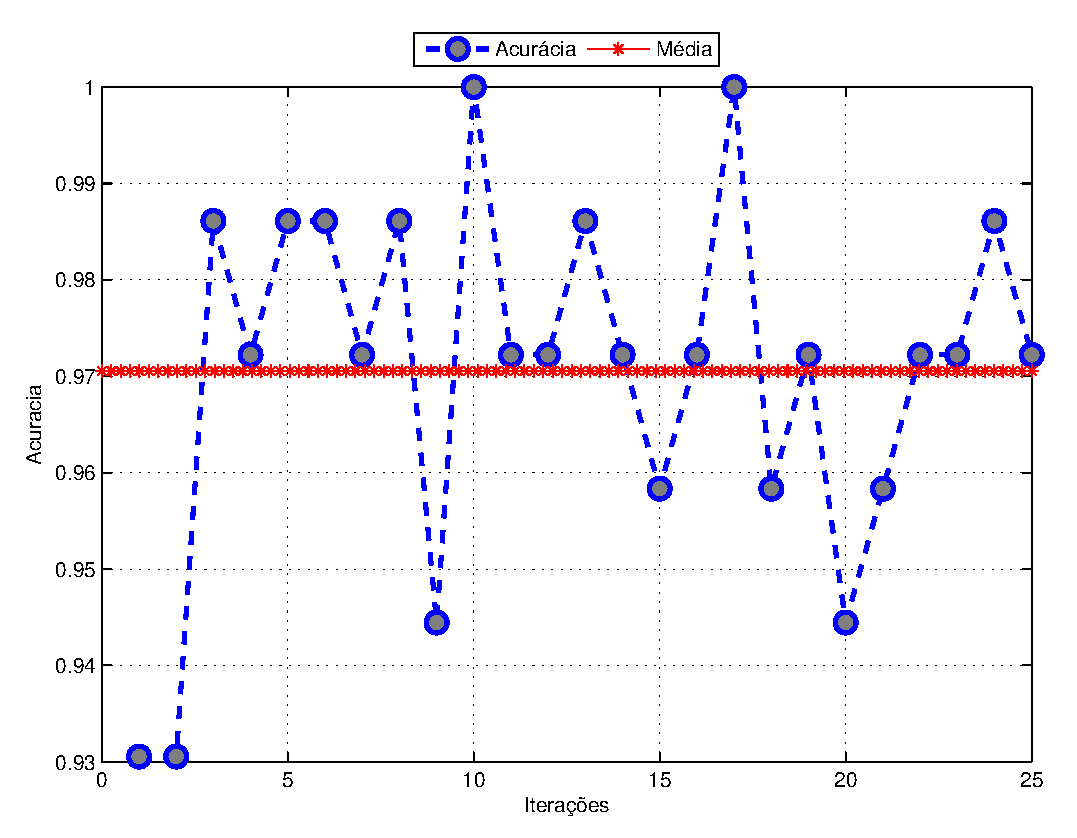
\includegraphics[width=0.4\textwidth]{Imagens/plotAccDerm_type4.eps}}

\caption{Resultados da Acurácia para Dermatologia.}
\label{fig:Figura3}
\end{figure}



\subsubsection{Coluna Vertebral}

\begin{figure}[H]
\centering

\subfigure[Quadrática]{ 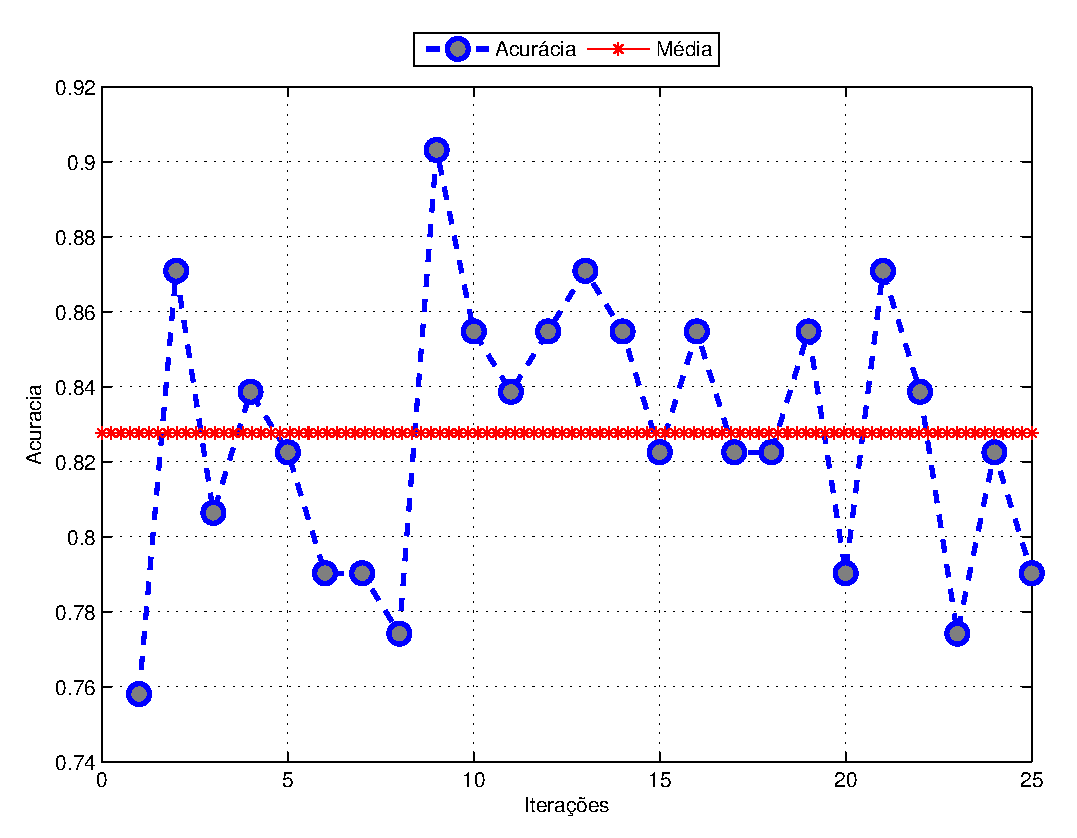
\includegraphics[width=0.4\textwidth]{Imagens/plotAccColumm_type1.eps}}
\subfigure[Linear]{ 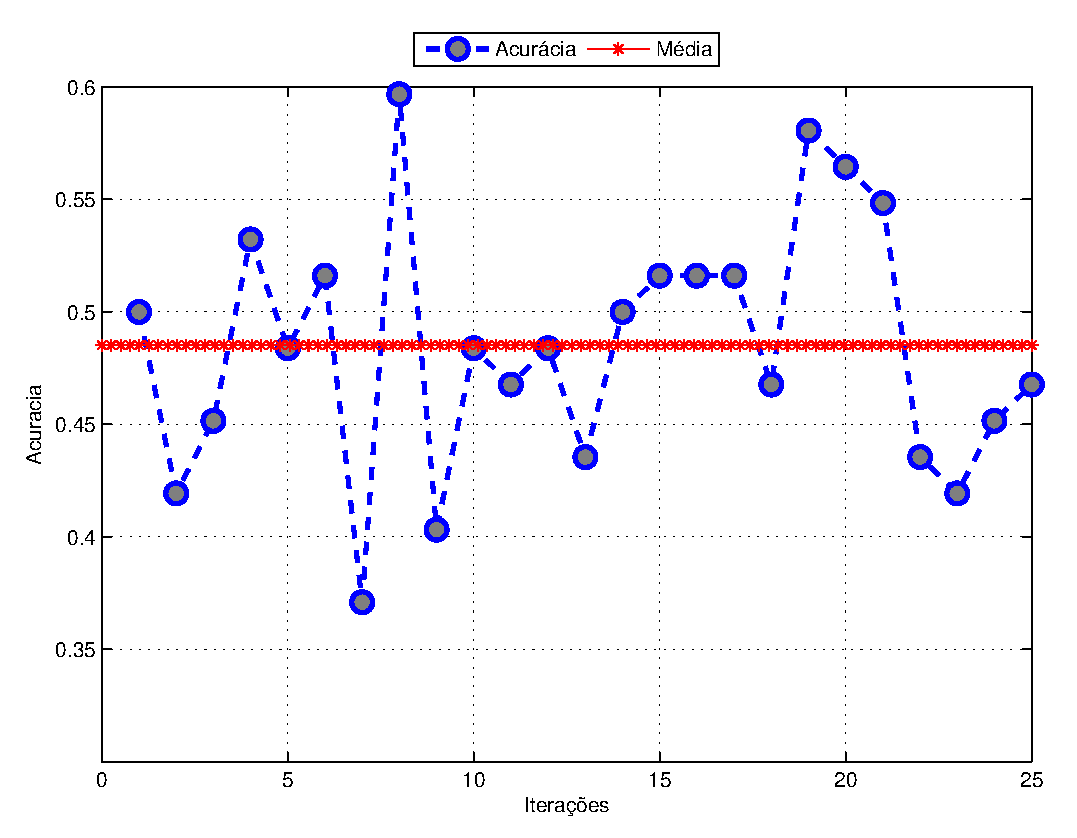
\includegraphics[width=0.4\textwidth]{Imagens/plotAccColumm_type2.eps}}
\subfigure[Distância Euclidiana]{ 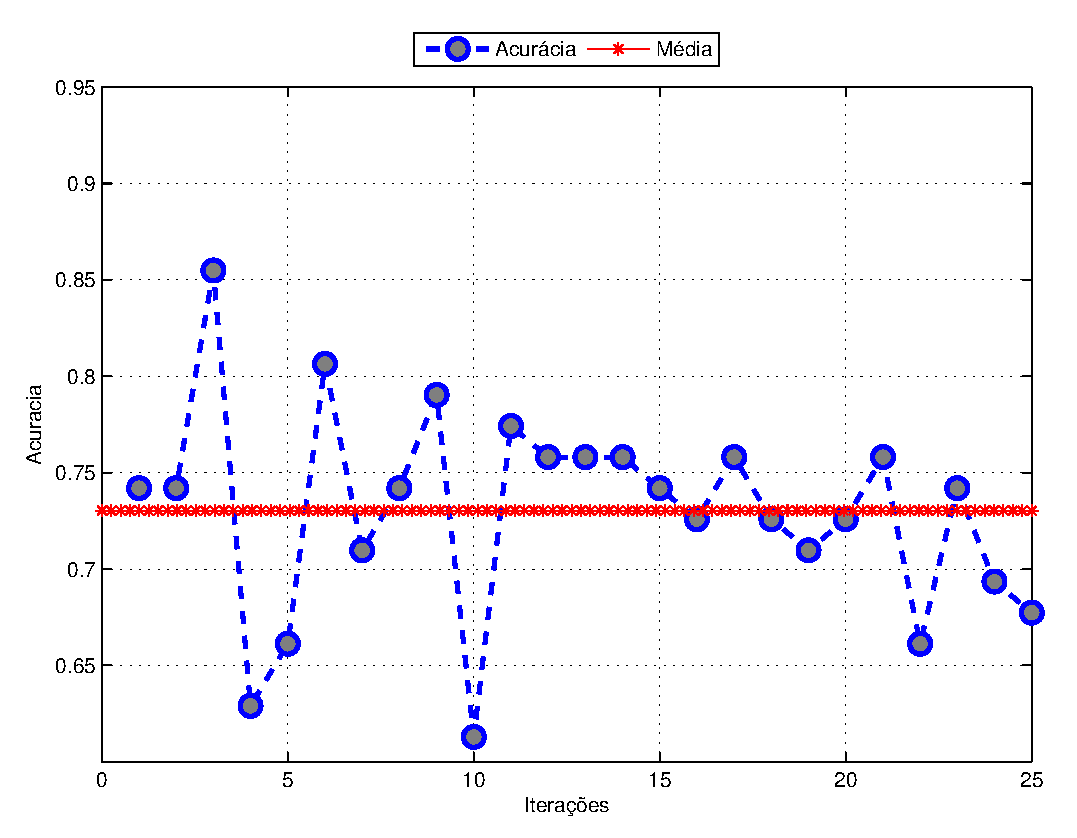
\includegraphics[width=0.4\textwidth]{Imagens/plotAccColumm_type3.eps}}
\subfigure[Mahalanobis]{ 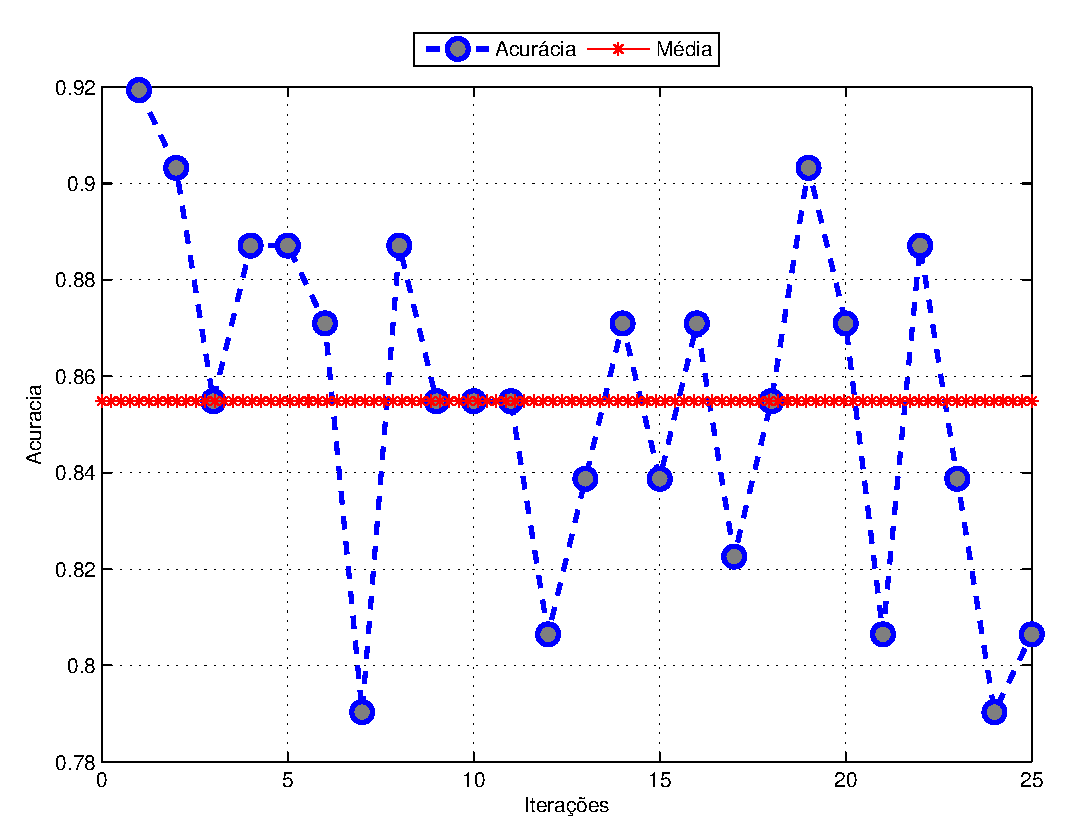
\includegraphics[width=0.4\textwidth]{Imagens/plotAccColumm_type4.eps}}

\caption{Resultados da Acurácia para Coluna Vertebral.}
\label{fig:Figura4}
\end{figure}



Na Tabela 1, mostra os resultados da acurácia média e desvio padrão para cada função discriminante de acordo com a base.

% Please add the following required packages to your document preamble:
% \usepackage{booktabs}
% \usepackage{multirow}
% \usepackage[table,xcdraw]{xcolor}
% If you use beamer only pass "xcolor=table" option, i.e. \documentclass[xcolor=table]{beamer}
\begin{table}[h]
\caption{Acurácia e Desvio Padrão para os classificadores Bayesiano.}
\begin{tabular}{@{}ccccc@{}}
\toprule
\multicolumn{2}{c}{}                                                                                                                                           & \textbf{Flor de Íris}          & \textbf{Dermatologia}          & \textbf{\begin{tabular}[c]{@{}c@{}}Coluna \\ Vertebral\end{tabular}} \\ \midrule
                                                                                           & \cellcolor[HTML]{EFEFEF}\textbf{Média}                            & \cellcolor[HTML]{EFEFEF}0.9840 & \cellcolor[HTML]{EFEFEF}0.9688 & \cellcolor[HTML]{EFEFEF}0.8277                                       \\ \cmidrule(l){2-5} 
\multirow{-2}{*}{\textbf{Quadrática}}                                                      & \textbf{\begin{tabular}[c]{@{}c@{}}Desvio \\ Padrão\end{tabular}} & 0.0217                         & 0.0197                         & 0.0365                                                               \\ \midrule
                                                                                           & \cellcolor[HTML]{EFEFEF}\textbf{Média}                            & \cellcolor[HTML]{EFEFEF}0.8493 & \cellcolor[HTML]{EFEFEF}0.9633 & \cellcolor[HTML]{EFEFEF}0.4851                                       \\ \cmidrule(l){2-5} 
\multirow{-2}{*}{\textbf{Linear}}                                                          & \textbf{\begin{tabular}[c]{@{}c@{}}Desvio \\ Padrão\end{tabular}} & 0.0739                         & 0.0203                         & 0.0558                                                               \\ \midrule
                                                                                           & \cellcolor[HTML]{EFEFEF}\textbf{Média}                            & \cellcolor[HTML]{EFEFEF}0.9253 & \cellcolor[HTML]{EFEFEF}0.9561 & \cellcolor[HTML]{EFEFEF}0.7303                                       \\ \cmidrule(l){2-5} 
\multirow{-2}{*}{\textbf{\begin{tabular}[c]{@{}c@{}}Distância \\ Euclidiana\end{tabular}}} & \textbf{\begin{tabular}[c]{@{}c@{}}Desvio \\ Padrão\end{tabular}} & 0.0433                         & 0.0249                         & 0.0540                                                               \\ \midrule
                                                                                           & \cellcolor[HTML]{EFEFEF}\textbf{Média}                            & \cellcolor[HTML]{EFEFEF}0.9826 & \cellcolor[HTML]{EFEFEF}0.9705 & \cellcolor[HTML]{EFEFEF}0.8548                                       \\ \cmidrule(l){2-5} 
\multirow{-2}{*}{\textbf{Mahalanobis}}                                                     & \textbf{\begin{tabular}[c]{@{}c@{}}Desvio \\ Padrão\end{tabular}} & 0.0195                         & 0.0185                         & 0,0360                                                               \\ \bottomrule
\end{tabular}
\end{table}

\subsection{Distribuição Gaussiana para Flor de Íris}

Levando em consideração a questão prática e teórica, da pra dizer que a distribuição Normal conhecida também como distribuição Gaussiana, é sem dúvida, a mais relevante distribuição estatística. Essa distribuição apresenta-se em formato de sino, unimodal, simétrica em relação a sua média, considerando a probabilidade de ocorrência, a área sob sua curva soma 100\%. Isso quer dizer que a probabilidade de uma observação assumir um valor entre dois pontos quaisquer é igual à área compreendida entre esses dois pontos. A seguir as imagens das Gaussianas para as 4 Funções Discriminantes.


\begin{figure}[H]
\centering

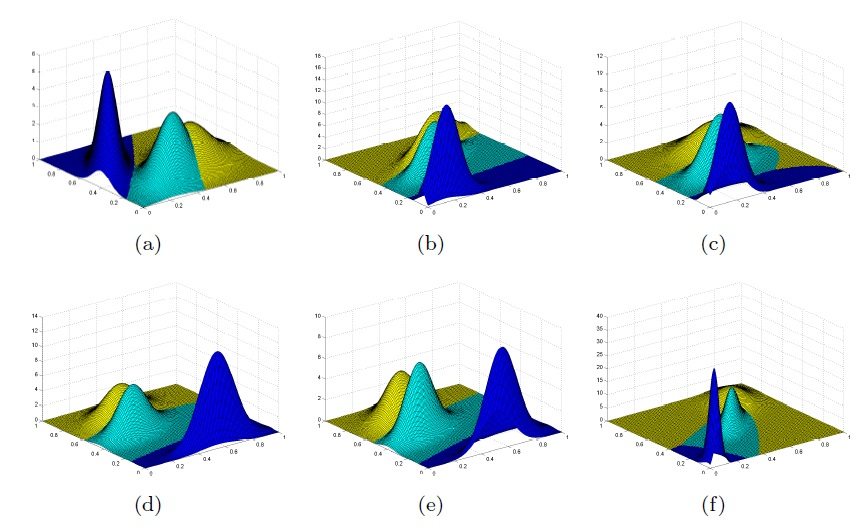
\includegraphics[height=7cm]{Imagens/plotGauss_type1.jpg}

\caption{Gaussiana Quadrática.}
\label{fig:Figura5}
\end{figure}


\begin{figure}[H]
\centering

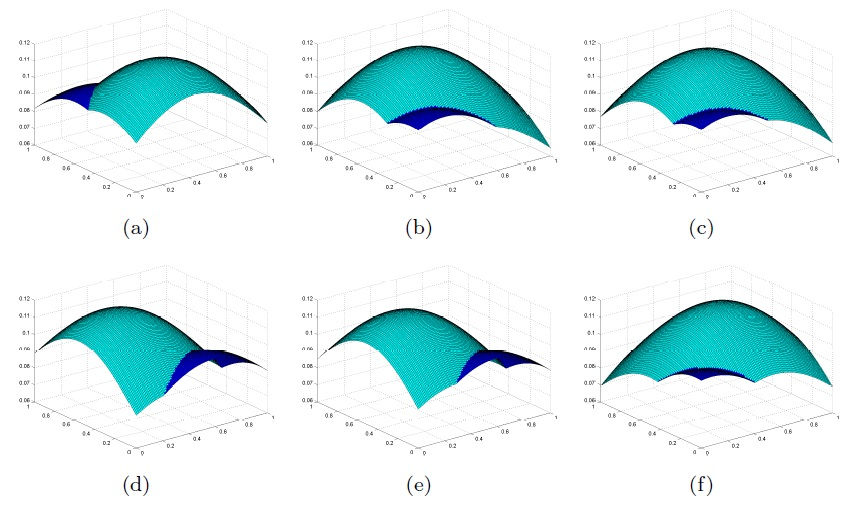
\includegraphics[height=7cm]{Imagens/plotGauss_type2.jpg}

\caption{Gaussiana Linear.}
\label{fig:Figura6}
\end{figure}


\begin{figure}[H]
\centering

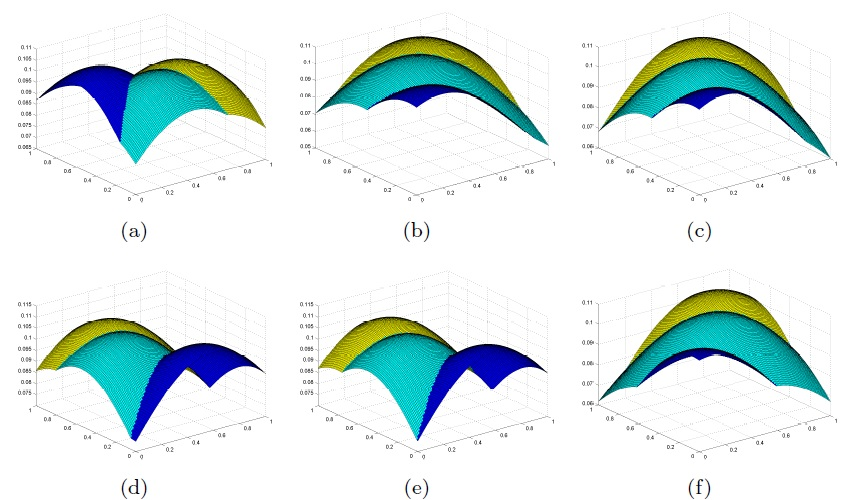
\includegraphics[height=7cm]{Imagens/plotGauss_type3.jpg}

\caption{Gaussiana da Distância Euclidiana.}
\label{fig:Figura7}
\end{figure}


\begin{figure}[H]
\centering

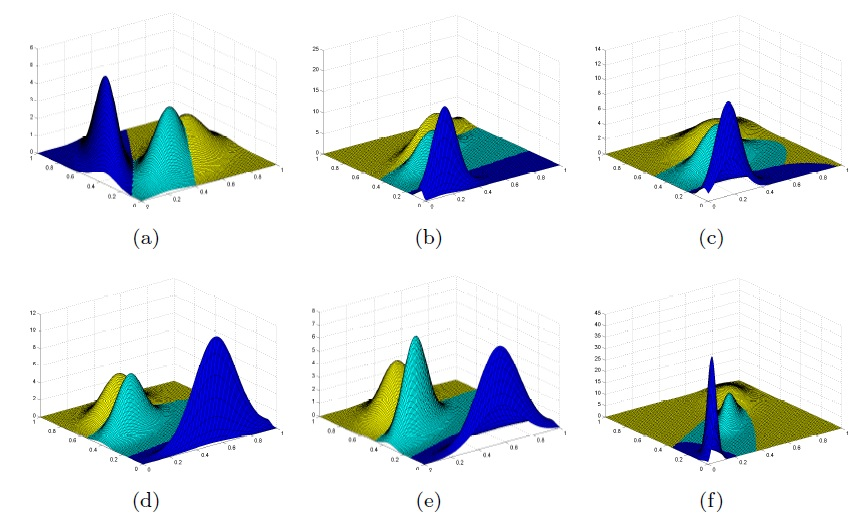
\includegraphics[height=7cm]{Imagens/plotGauss_type4.jpg}

\caption{Gaussiana de Mahalanobis.}
\label{fig:Figura8}
\end{figure}


\subsection{Região de Decisão para Flor de Íris}

Em geral, um classificador particiona o espaço de características em volumes designados regiões de decisão. Todos os vectores de características no interior de uma região de decisão são atribuídos à mesma categoria.\\


O efeito de qualquer regra de decisão é dividir o espaco de características em c regiões de decisão R1, R2, $\cdots$, Rc . Se $g_i (x) > g_j(x)  \forall_j \neq i$, então x está em $R_i$ . \\

As regiões são separadas por superfícies de decisão, isto é, as superfícies formadas pelos pontos que pertencem a mais de uma funcão discriminante (interseção entre as superfícies).\\

Para as superfícies de decisão Quadrática, assumem a forma de elipsóides, parábolas e hipérboles no espaço de separação, ver figura \ref{fig:Figura9}.


\begin{figure}[H]
\centering

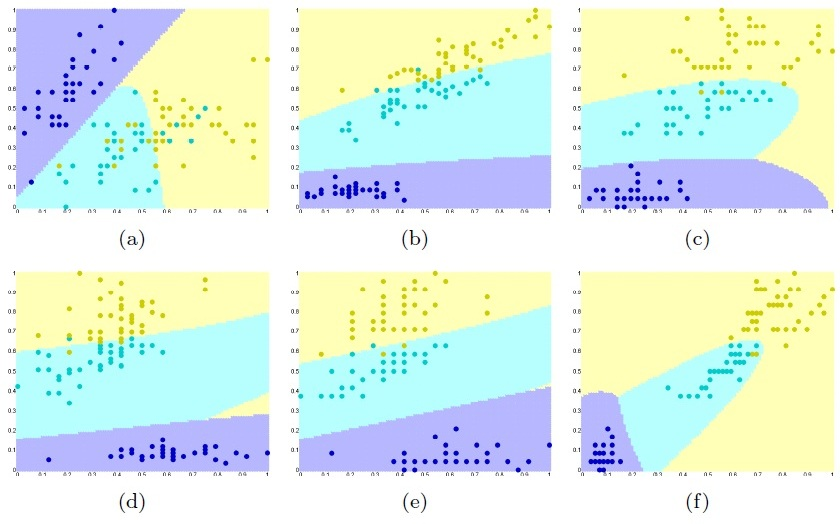
\includegraphics[height=7cm]{Imagens/decisionboundary_type1.jpg}

\caption{Região de Decisão Quadrática.}
\label{fig:Figura9}
\end{figure}

Para as superfícies de decisão Linear, assumem a forma de hiperplano no espaço de separação, ver figura \ref{fig:Figura11}.

\begin{figure}[H]
\centering

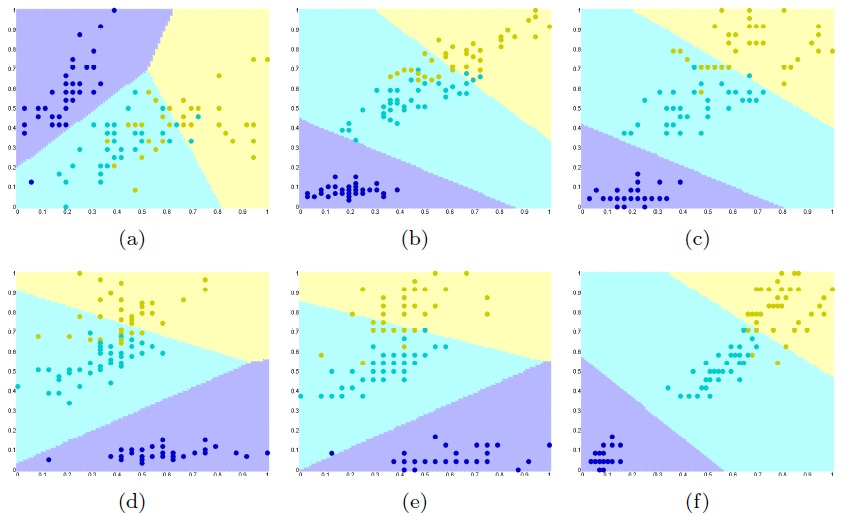
\includegraphics[height=7cm]{Imagens/decisionboundary_type2.jpg}

\caption{Região de Decisão Linear.}
\label{fig:Figura11}
\end{figure}


Para as superfícies de decisão Distância Euclidiana, assumem a forma de hiperplano, com pequenas variações em relação superfícies de separação linear, ver figura \ref{fig:Figura12}.


\begin{figure}[H]
\centering

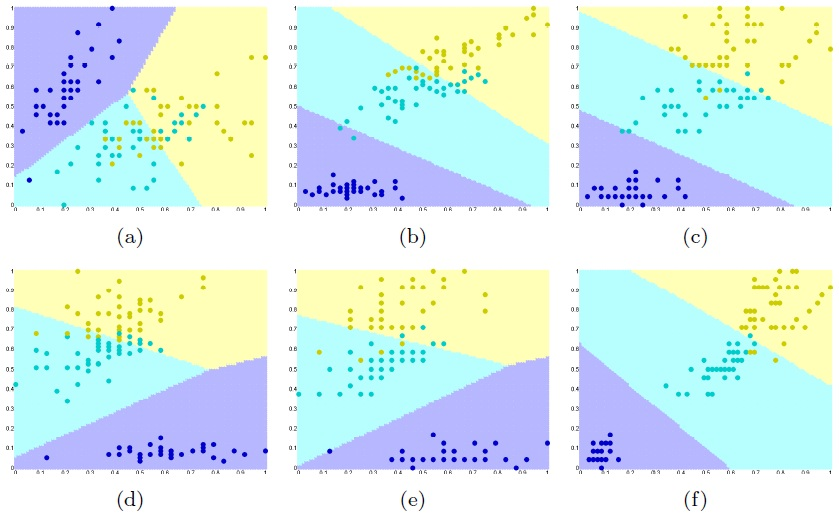
\includegraphics[height=7cm]{Imagens/decisionboundary_type3.jpg}

\caption{Região de Decisão Distância Euclidiana.}
\label{fig:Figura12}
\end{figure}


Para as superfícies de decisão de Mahalanobis, são formadas por hiper-elipsóides, com pequenas variações em relação superfícies de decisão Quadrática, ver figura \ref{fig:Figura13}.


\begin{figure}[H]
\centering

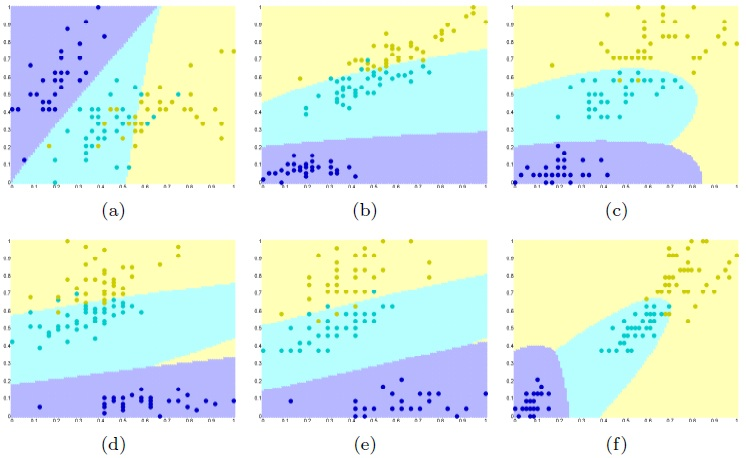
\includegraphics[height=7cm]{Imagens/decisionboundary_type4.jpg}

\caption{Região de Decisão de Mahalanobis.}
\label{fig:Figura13}
\end{figure}


\section{Conclusões}

As técnicas de Aprendizagem de Máquina tem sido cada vez mais usadas para resolver todos os tipos de problemas da computação. São vários os motivos pelo seu uso, tendo destaque a sua maior flexibilidade, adaptabilidade e bons resultados gerado. \\

Neste relatório, foi apresentado e implementado o classificador de Bayes demonstrando que o aprendizado bayesiano é uma abordagem bastante simples e robusta, com valores de acurácia bem satisfotório e minimizando as taxas de erro. 


\begin{thebibliography}{1}

\bibitem{IEEEhowto:kopka}
[UCI15] Uci machine learning repository, 2015. Disponível em: <http:// archive.ics.uci.edu/ml/>.

\bibitem{IEEEhowto:kopka}
Frutuoso, R. L. Identificação de Órgãos foliares utilizando as wavelets de daubechies. XIV Workshop de Informática Médica, FCT/UNESP, v. 1, n. 1, p. 211–126, 2013. ISSN none. Disponível em: <http://www.lbd.dcc.ufmg.br/colecoes/wvc/2010/0037.pdf>. Citado na página 8.

\bibitem{IEEEhowto:kopka}
Kohavi, R. A study of cross-validation and bootstrap for accuracy estimation and model selection. In: International joint Conference on artificial intelligence. [S.l.: s.n.], 1995. v. 14, p. 1137–1145.

\bibitem{IEEEhowto:kopka}
Scaranti, A. ; Bernardi, R. ; Plotze, R. O.. (2010) “Identificação de Órgãos Foliares Utilizando as Wavelets de Daubechies”. In: WVC'2010 - VI Workshop de Visão Computacional.

\bibitem{IEEEhowto:kopka}
[DeGroot, 1989] DeGroot, M. H. (1989). Probability and Statistics. Addison-Wesley, 2nd edition.

\bibitem{IEEEhowto:kopka}
[Duda et al., 2001] Duda, R. O., Hart, P. E., and Stork, D. G. (2001). Pattern Classification. John Wiley and Sons.

\bibitem{IEEEhowto:kopka}
[Kohn, 1999] Kohn, A. F. (1999). Reconhecimento de Padrões - Uma Abordagem Estatística. EPUSP.

\bibitem{IEEEhowto:kopka}
[Meyer, 1969] Meyer, P. L. (1969). Probabilidade - Aplicações à Estaística. Ao Livro Técnico S.A. Versão traduzida do original em inglês.


\bibitem{pichiliani2008conversando}
  {Conversando Sobre Banco De Dados},
  {Pichiliani, M.C.},
  {Clube de Autores},
  {2008}


\end{thebibliography}


%%%%%%%%    Apêndice  %%%%%%%%
\newpage
\appendix
\section{Apêndice}

\title{\textbf{Código para implementação em MATLAB}}


\begin{description}
\item[] 
\end{description}

\textbf{Bayes}
\lstinputlisting{Codigo/runbayes.m}

\newpage

\textbf{Treino Bayes}
\lstinputlisting{Codigo/bayesTraining.m}

\newpage

\begin{description}
\item[] 
\end{description}

\textbf{Teste Bayes}
\lstinputlisting{Codigo/bayesTest.m}


\begin{description}
\item[] 
\end{description}

\newpage

\textbf{Plot das Características}
\lstinputlisting{Codigo/plotLabels.m}

\begin{description}
\item[] 
\end{description}

\newpage

\textbf{Plot Região de Decisão}
\lstinputlisting{Codigo/deciosionregion.m}


\end{document}